%%%%%%%%%%%%%%%%%%%%%%%%%%%%%%%%%%%%%%%%%
% FRI Data Science_report LaTeX Template
% Version 1.0 (28/1/2020)
% 
% Jure Demšar (jure.demsar@fri.uni-lj.si)
%
% Based on MicromouseSymp article template by:
% Mathias Legrand (legrand.mathias@gmail.com) 
% With extensive modifications by:
% Antonio Valente (antonio.luis.valente@gmail.com)
%
% License:
% CC BY-NC-SA 3.0 (http://creativecommons.org/licenses/by-nc-sa/3.0/)
%
%%%%%%%%%%%%%%%%%%%%%%%%%%%%%%%%%%%%%%%%%


%----------------------------------------------------------------------------------------
%	PACKAGES AND OTHER DOCUMENT CONFIGURATIONS
%----------------------------------------------------------------------------------------
\documentclass[fleqn,moreauthors,10pt]{ds_report}
\usepackage[english]{babel}
\usepackage{float}
\usepackage{array}

\graphicspath{{fig/}}




%----------------------------------------------------------------------------------------
%	ARTICLE INFORMATION
%----------------------------------------------------------------------------------------

% Header
\JournalInfo{FRI Natural language processing course 2024}

% Interim or final report
\Archive{Project report} 
%\Archive{Final report} 

% Article title
\PaperTitle{Parameter-Efficient Fine-Tuning of Language Models} 

% Authors (student competitors) and their info
\Authors{Lena Trnovec, Tjaša Domadenik, Anže Oblak}

% Advisors
\affiliation{\textit{Advisors: Aleš Žagar}}

% Keywords
\Keywords{Fine-tuning ...}
\newcommand{\keywordname}{Keywords}


%----------------------------------------------------------------------------------------
%	ABSTRACT
%----------------------------------------------------------------------------------------

\Abstract{
The abstract goes here. The abstract goes here. The abstract goes here. The abstract goes here. The abstract goes here. The abstract goes here. The abstract goes here. The abstract goes here. The abstract goes here. The abstract goes here. The abstract goes here. The abstract goes here. The abstract goes here. The abstract goes here. The abstract goes here. The abstract goes here. The abstract goes here. The abstract goes here. The abstract goes here. The abstract goes here. The abstract goes here. The abstract goes here. The abstract goes here. The abstract goes here. The abstract goes here. The abstract goes here.
}

%----------------------------------------------------------------------------------------

\begin{document}

% Makes all text pages the same height
\flushbottom 

% Print the title and abstract box
\maketitle 

% Removes page numbering from the first page
\thispagestyle{empty} 

%----------------------------------------------------------------------------------------
%	ARTICLE CONTENTS
%----------------------------------------------------------------------------------------

\section*{Introduction}
Transformer-based pretrained language models (PLMs) have revolutionized natural language processing (NLP) tasks, by demonstrating remarkable success in understanding and generating human-like text. To fully harness their potential, fine-tuning is employed to adapt the models to task specific data and enhance their performance. However, traditional fine-tuning involves updating all the pretrained parameters of PLM, which requires substantial computational resources. With PLMs continuing to grow, the number of parameters increases even further and so do the computational demands, which becomes a significant challenge. In response to that, various parameter efficient fine-tunning (PEFT) techniques have emerged, as a viable solution to compensate for the tremendous computational cost, while still maintaining comparable performance to the full fine-tuning.

One of the commonly used techniques is additive fine-tuning, which adds new trainable parameters to pre-trained models. It can be divided into adapter and soft prompt-based methods. Adapters insert small modules between transformer layers in the existing model structure, while soft prompts add trainable vectors to the model inputs, subtly directing the output with minimal changes. In previous research a variety of adapter methods were explored. Some of the notable ones are parallel adapter \cite{he2021towards} which integrates the network in parallel with the feed-forward layer and attention layer and AdapterDrop \cite{ruckle2020adapterdrop} which selectively removes adapters which are not important to the given task. Both methods build upon the foundational concept discussed in \cite{houlsby2019parameter} and present valuable case studies for our investigation. We will also examine prefix-tuning, a prompt-based method \cite{li2021prefix}. This approach focuses on optimizing a task-specific set of parameters, known as a \textit{prefix}. It modifies only about 0.1\% of the parameters in comparison to traditional fine-tuning. Despite this, it achieves comparable performance in datasets with full data settings, making it an interesting candidate for comparison.

Another method, known as Low-Rank Adaptation (LoRA), is a reparameterized fine-tuning method that specifically targets the model's weight matrices. It introduces low-rank matrices that interact with the original weights to apply precise updates, rather than altering or adding extensive new parameters \cite{hu_lora_2021}. This strategy allows for the efficient adaptation of PLMs by modifying a relatively small subset of parameters, thereby mitigating the computational load while still achieving competitive performance \cite{zeng_expressive_2024, dinh_lift_2022}.

Another possible approach is hybrid fine-tuning, which tries to combine various PEFT approaches, such as adapter, prefix-tuning and LoRA. This way it leverages the strengths of each method and mitigates their weaknesses and consequently achieves improved overall performance compared to individual PEFT methods. The work in this area is classified into two approaches: Manual Combination and Automatic Combination. The first one involves manually combining multiple PEFT methods by sophisticated design. On the other hand Automatic Combination incorporates PEFT methods automatically via structure search and because of that it typically requires more time and cost. 
In one of the previous articles \cite{mao2021unipelt} authors proposed a method called UniPELT which incorporates sequential adapter, prefix-tuning, and LoRA via a gating mechanism. The mechanism controls the activation of each submodule, dynamically assigning higher weights to submodules that make positive contributions to a given task. The method requires more parameters and inference time than adapter, prefix-tuning, and LoRA, but achieves better performance than those individual methods. Another article \cite{zhou2023autopeft}, presents method AutoPEFT that integrates sequential adapter, parallel adapter and prefix tuning into the transformer block. The method also uses Bayesian optimization approach to automatically search for an appropriate architecture of neural network that activates certain layers to incorporate these PEFT modules.

	% These latex files are intended to serve as a the template for the NLP course at FRI.  The template is adapted from the FRI Data Science Project Competition. template  If you find mistakes in the template or have problems using it, please consult Jure Demšar (\href{mailto:jure.demsar@fri.uni-lj.si}{jure.demsar@fri.uni-lj.si}).
	
	% In the Introduction section you should write about the relevance of your work (what is the purpose of the project, what will we solve) and about related work (what solutions for the problem already exist). Where appropriate, reference scientific work conducted by other researchers. For example, the work done by Demšar et al. \cite{Demsar2016BalancedMixture} is very important for our project. The abbreviation et al. is for et alia, which in latin means and others, we use this abbreviation when there are more than two authors of the work we are citing. If there are two authors (or if there is a single author) we just write down their surnames. For example, the work done by Demšar and Lebar Bajec \cite{Demsar2017LinguisticEvolution} is also important for successful completion of our project.


%------------------------------------------------

\section*{Methods}
% \begin{itemize}
    % \item Which pretrained language model to use?
    % \begin{itemize}
    %     \item \textbf{BERT} (Bidirectional Encoder Representations from Transformers) - highly successful across a wide range of NLP tasks, well-suited for understanding tasks but can be adapted for generation tasks as well.
    %     \item \textbf{GPT} (Generative Pre-trained Transformer) - excels in generation tasks and can perform admirably in understanding tasks when fine-tuned or used with prompting techniques.
    %     \item \textbf{T5} (Text-to-Text Transfer Transformer) - versatile for both understanding and generation tasks.
    % \end{itemize} 
    
    % (T5 seems like the best choice, TBD...). First testing on smaller models then onto larger ones (colab or SLING).
    Pretrained models we will be using:
    \begin{itemize}
        \item \textbf{google-bert/bert-base-uncased:} Pretrained mo\-del on English language using a masked language modeling (MLM) objective. This model is uncased, which means that it does not make a difference between english and English. It's good model for our starting implementations, because it's a bit smaller.
        \item \textbf{EMBEDDIA/crosloengual-bert:} A trilingual mo\-del, using bert-base architecture, trained on Croatian, Slovenian, and English corpora. We opted for this model due to its potential for good performance, since it is already trained on Slovenian corpora.
    \end{itemize}
    
    PEFT approaches used: 
    \begin{itemize}
        \item \textbf{Prompt-Tuning:} Fine-tunes a small set of task-specific tokens appended to the input without altering the original model parameters.
        \item \textbf{LoRA:} Modifies the weight matrices of a model by applying low-rank updates, preserving the original parameters while adapting to new tasks.
        \item \textbf{LoHa:} Is similar to LoRA except it approximates the large weight matrix with more low-rank matrices and combines them with the Hadamard product. The method is supposed to be even more parameter-efficient than LoRA, yet it achieves performance levels comparable to it.
     \end{itemize}
    
    We decided to use \textbf{Slovene SuperGLUE} dataset, from Slobench, because it provides multiple different tasks, which are as follows:
    \begin{itemize}
        \item \textbf{BoolQ:} determine whether a given passage contains the answer to a yes/no question.
        \item \textbf{CB:} determine the commitment of a statement to a specific target.
        \item \textbf{COPA:} presents a premise and requires choosing the correct alternative explanation or cause.
        \item \textbf{MultiRC:} answering multiple-choice questions based on a given passage, with each question having multiple correct answers.
        \item \textbf{RTE:} determine whether one text implies another, often categorized as entailment, contradiction, or neutral.
        \item \textbf{WSC:} test machines' understanding of pronouns and their antecedents in a sentence.
     \end{itemize}
    
    % At least 5 different datasets that cover various natural language understanding skills (commonsense reasoning, coreference resolution, text summarization, etc.) and supervised learning settings (classification \& generation).
    
    % From SloBENCH?
    % \begin{itemize}
    %     \item https://slobench.cjvt.si/leaderboard/view/9 (sequence classification) (Given a premise and a hypothesis, the task is to detect whether the hypothesis entails, contradicts, or is neutral in relation to the premise.)
    %     \item https://slobench.cjvt.si/leaderboard/view/12 (token classification) (Given tokenized text, the task is to annotate each token with an appropriate label.)
    %     \item https://slobench.cjvt.si/leaderboard/view/7 (conditional generation, slo-eng translation)
    %     \item https://slobench.cjvt.si/leaderboard/view/8 (conditional generation, slo-eng translation)
    % \end{itemize}
    
    Metrics: 
    \begin{itemize}
        \item \textbf{accuracy}
        \item \textbf{F1 score}
     \end{itemize}

    Previously described methods are not necessarily final. We may change some of them, in order to achieve a manageable set of testing combinations.
    
% \end{itemize}

% \subsection*{Equations}

% %You can write equations inline, e.g. $\cos\pi=-1$, $E = m \cdot c^2$ and $\alpha$, or you can include them as separate objects. The Bayes’s rule is stated mathematically as:

% %\begin{equation}
% %	P(A|B) = \frac{P(B|A)P(A)}{P(B)},
% %	\label{eq:bayes}
% %\end{equation}

% %where $A$ and $B$ are some events. You can also reference it -- the equation \ref{eq:bayes} describes the Bayes's rule.

% %\subsection*{Lists}

% %We can insert numbered and bullet lists:

% % the [noitemsep] option makes the list more compact
% %\begin{enumerate}[noitemsep] 
% %	\item First item in the list.
% %	\item Second item in the list.
% %	\item Third item in the list.
% %\end{enumerate}

% %\begin{itemize}[noitemsep] 
% %	\item First item in the list.
% %	\item Second item in the list.
% %	\item Third item in the list.
% %\end{itemize}

% %We can use the description environment to define or describe key terms and phrases.

% %\begin{description}
% %	\item[Word] What is a word?.
% %	\item[Concept] What is a concept?
% %	\item[Idea] What is an idea?
% %\end{description}


% %\subsection*{Random text}

% %This text is inserted only to make this template look more like a proper report. Lorem ipsum dolor sit amet, consectetur adipiscing elit. Etiam blandit dictum facilisis. Lorem ipsum dolor sit amet, consectetur adipiscing elit. Interdum et malesuada fames ac ante ipsum primis in faucibus. Etiam convallis tellus velit, quis ornare ipsum aliquam id. Maecenas tempus mauris sit amet libero elementum eleifend. Nulla nunc orci, consectetur non consequat ac, consequat non nisl. Aenean vitae dui nec ex fringilla malesuada. Proin elit libero, faucibus eget neque quis, condimentum laoreet urna. Etiam at nunc quis felis pulvinar dignissim. Phasellus turpis turpis, vestibulum eget imperdiet in, molestie eget neque. Curabitur quis ante sed nunc varius dictum non quis nisl. Donec nec lobortis velit. Ut cursus, libero efficitur dictum imperdiet, odio mi fermentum dui, id vulputate metus velit sit amet risus. Nulla vel volutpat elit. Mauris ex erat, pulvinar ac accumsan sit amet, ultrices sit amet turpis.

% %Phasellus in ligula nunc. Vivamus sem lorem, malesuada sed pretium quis, varius convallis lectus. Quisque in risus nec lectus lobortis gravida non a sem. Quisque et vestibulum sem, vel mollis dolor. Nullam ante ex, scelerisque ac efficitur vel, rhoncus quis lectus. Pellentesque scelerisque efficitur purus in faucibus. Maecenas vestibulum vulputate nisl sed vestibulum. Nullam varius turpis in hendrerit posuere.


% %\subsection*{Figures}

% %You can insert figures that span over the whole page, or over just a single column. The first one, \figurename~\ref{fig:column}, is an example of a figure that spans only across one of the two columns in the report.

% %\begin{figure}[ht]\centering
% %	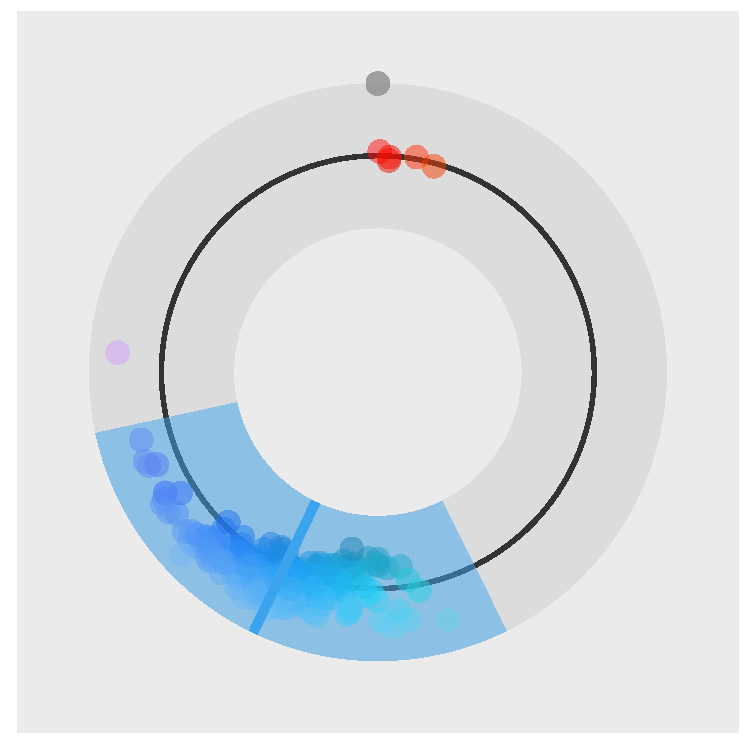
\includegraphics[width=\linewidth]{single_column.pdf}
% %	\caption{\textbf{A random visualization.} This is an example of a figure that spans only across one of the two columns.}
% %	\label{fig:column}
% %\end{figure}

% %On the other hand, \figurename~\ref{fig:whole} is an example of a figure that spans across the whole page (across both columns) of the report.

% % \begin{figure*} makes the figure take up the entire width of the page
% %\begin{figure*}[ht]\centering 
% %	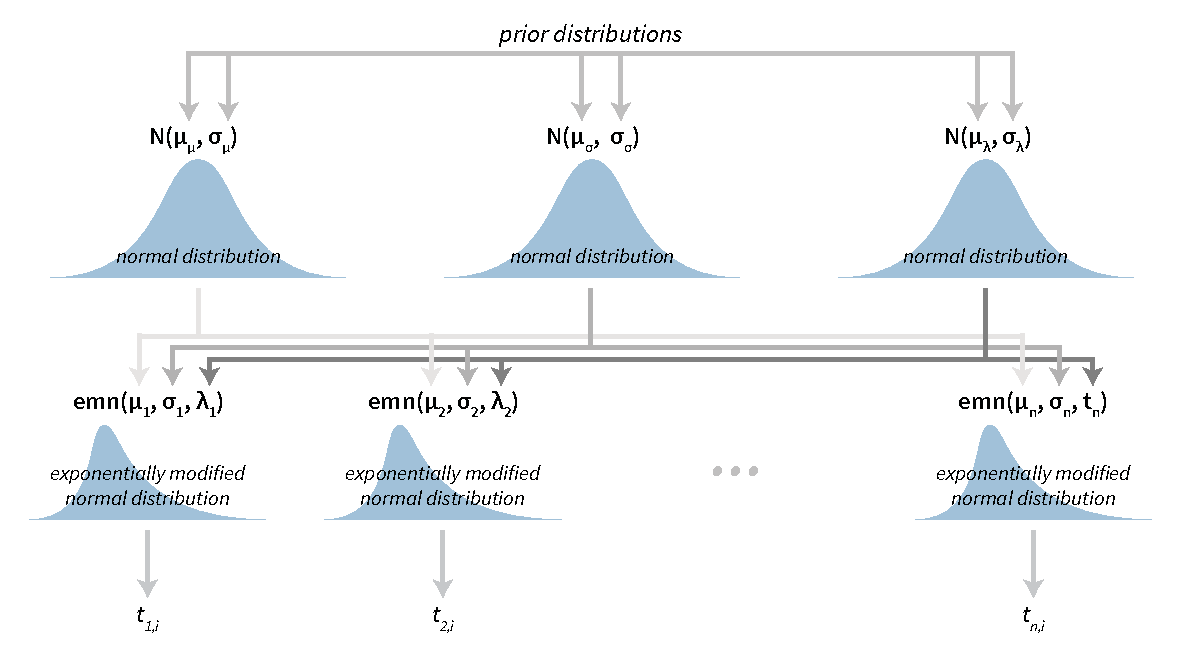
\includegraphics[width=\linewidth]{whole_page.pdf}
% %	\caption{\textbf{Visualization of a Bayesian hierarchical model.} This is an example of a figure that spans the whole width of the report.}
% %	\label{fig:whole}
% %\end{figure*}


% \subsection*{Tables}

% Use the table environment to insert tables.

% \begin{table}[hbt]
% 	\caption{Table of grades.}
% 	\centering
% 	\begin{tabular}{l l | r}
% 		\toprule
% 		\multicolumn{2}{c}{Name} \\
% 		\cmidrule(r){1-2}
% 		First name & Last Name & Grade \\
% 		\midrule
% 		John & Doe & $7.5$ \\
% 		Jane & Doe & $10$ \\
% 		Mike & Smith & $8$ \\
% 		\bottomrule
% 	\end{tabular}
% 	\label{tab:label}
% \end{table}


% \subsection*{Code examples}

% You can also insert short code examples. You can specify them manually, or insert a whole file with code. Please avoid inserting long code snippets, advisors will have access to your repositories and can take a look at your code there. If necessary, you can use this technique to insert code (or pseudo code) of short algorithms that are crucial for the understanding of the manuscript.

% \lstset{language=Python}
% \lstset{caption={Insert code directly from a file.}}
% \lstset{label={lst:code_file}}
% \lstinputlisting[language=Python]{code/example.py}

% \lstset{language=R}
% \lstset{caption={Write the code you want to insert.}}
% \lstset{label={lst:code_direct}}
% \begin{lstlisting}
% import(dplyr)
% import(ggplot)

% ggplot(diamonds,
% 	   aes(x=carat, y=price, color=cut)) +
%   geom_point() +
%   geom_smooth()
% \end{lstlisting}

% ------------------------------------------------

\section*{Results}

Up to this point, we tried to fine tune some models on different tasks from the dataset. The results are shown in tables \ref{table:boolq_performance}, \ref{table:cb_performance} and \ref{table:copa_performance}. During the process of training and fine tuning, we ran into some problems, as the models achieved very bad performance in some cases. Despite thorough debugging and testing of our implementations, we are still not sure if there is a bug in our code or if the models really just struggle with these tasks.

\begin{table}[H]
\begin{center}
\begin{tabular}{|*{1}{>{\centering\arraybackslash}m{1.7 cm}}|*{1}{>{\centering\arraybackslash}m{2.2 cm}}|*{1}{>{\centering\arraybackslash}m{1.3cm}}|*{1}{>{\centering\arraybackslash}m{1.2cm}}|}
\hline
\textbf{Method} & \textbf{Model} & \textbf{Accuracy} & \textbf{f1} \\

\hline
 fine tuning only & bert-base-uncased & 0.72 &   0.73\\
\hline
 prompt tuning & bert-base-uncased & 0.83 &   0.79\\
\hline
LoHa & bert-base-uncased & 0.78 & 0.68\\
\hline
LoRa & bert-base-uncased & 0.78 & 0.68\\
\hline
\hline
 fine tuning only & crosloengual-bert & 0.83 &   0.82\\
\hline
 prompt tuning & crosloengual-bert & 0.78 &   0.68\\
\hline
LoHa & crosloengual-bert & 0.83 & 0.82\\
\hline
LoRa & crosloengual-bert & 0.78 & 0.68\\
\hline

\end{tabular}
\end{center}
\caption{BoolQ task results on evaluation split of the dataset.}
\label{table:boolq_performance}
\end{table}



\begin{table}[H]
\begin{center}
\begin{tabular}{|*{1}{>{\centering\arraybackslash}m{1.7 cm}}|*{1}{>{\centering\arraybackslash}m{2.2 cm}}|*{1}{>{\centering\arraybackslash}m{1.3cm}}|*{1}{>{\centering\arraybackslash}m{1.2cm}}|}
\hline
\textbf{Method} & \textbf{Model} & \textbf{Accuracy} & \textbf{f1} \\

\hline
 fine tuning only & bert-base-uncased & 0.36 &  0.24\\
\hline
 prompt tuning & bert-base-uncased & 0.32 &  0.15\\
\hline
LoHa & bert-base-uncased & 0.32 &  0.15\\
\hline
LoRa & bert-base-uncased & 0.32 &  0.15\\
\hline
\hline
 fine tuning only & crosloengual-bert & 0.68 &  0.64\\
\hline
 prompt tuning & crosloengual-bert & 0.32 &  0.15\\
\hline
LoHa & crosloengual-bert & 0.32 &  0.15\\
\hline
LoRa & crosloengual-bert & 0.32 &  0.15\\
\hline

\end{tabular}
\end{center}
\caption{CB task results on evaluation split of the dataset.}
\label{table:cb_performance}
\end{table}


\begin{table}[H]
\begin{center}
\begin{tabular}{|*{1}{>{\centering\arraybackslash}m{1.7 cm}}|*{1}{>{\centering\arraybackslash}m{2.2 cm}}|*{1}{>{\centering\arraybackslash}m{1.3cm}}|*{1}{>{\centering\arraybackslash}m{1.2cm}}|}
\hline
\textbf{Method} & \textbf{Model} & \textbf{Accuracy} & \textbf{f1} \\

\hline
 fine tuning only & bert-base-uncased & 0.55 & 0.39\\
\hline
LoHa & bert-base-uncased & 0.52 & 0.52\\
\hline
LoRa & bert-base-uncased & 0.50 & 0.49\\
\hline
\hline
 fine tuning only & crosloengual-bert & 0.51 & 0.49\\
\hline
LoHa & crosloengual-bert & 0.58 & 0.58\\
\hline
LoRa & crosloengual-bert & 0.49 & 0.49\\
\hline


\end{tabular}
\end{center}
\caption{COPA task results on evaluation split of the dataset.}
\label{table:copa_performance}
\end{table}

% Use the results section to present the final results of your work. Present the results in a objective and scientific fashion. Use visualisations to convey your results in a clear and efficient manner. When comparing results between various techniques use appropriate statistical methodology.



%------------------------------------------------

\section*{Discussion}

TODO
% Use the Discussion section to objectively evaluate your work, do not just put praise on everything you did, be critical and exposes flaws and weaknesses of your solution. You can also explain what you would do differently if you would be able to start again and what upgrades could be done on the project in the future.


%------------------------------------------------

\section*{Acknowledgments}
TODO
% Here you can thank other persons (advisors, colleagues ...) that contributed to the successful completion of your project.


%----------------------------------------------------------------------------------------
%	REFERENCE LIST
%----------------------------------------------------------------------------------------
\bibliographystyle{unsrt}
\bibliography{report}


\end{document}